% !TeX encoding = UTF-8
\documentclass[12pt,A4paper,titlepage]{article}
\usepackage[spanish]{babel}
\usepackage[utf8]{inputenc} %Este paquete permite poner acentos directamente y ees
\usepackage[T1]{fontenc}
\usepackage{amsmath}
\usepackage{graphicx}%[pdftex]
\usepackage{graphicx, wrapfig}
\usepackage{fancyhdr}
\usepackage{anysize}
\usepackage{verbatim}
\usepackage[dvips,final]{epsfig}
\usepackage{epstopdf}
\usepackage{colortbl}
\usepackage{listings}
\usepackage{float}
\usepackage{color}
\marginsize{2.5cm}{2.5cm}{2.5cm}{2.5cm}
\usepackage{fancyhdr}
\pagestyle{fancy}
\fancyhf{}
\fancyhead[LO]{Arquitectura de Computadoras}
\fancyfoot[LE,RO]{\thepage}
\fancyfoot[LO]{Aagaard Martín - Navarro Matias}
\renewcommand{\footrulewidth}{0.4pt}


%\graphicspath{{figuras/}}

%defiino un estilo de ingreso de codigo
\definecolor{codegreen}{rgb}{0,0.6,0}
\definecolor{codegray}{rgb}{0.5,0.5,0.5}
\definecolor{codepurple}{rgb}{0.58,0,0.82}
\definecolor{backcolour}{rgb}{0.95,0.95,0.92}
 
\lstdefinestyle{mystyle}{
    backgroundcolor=\color{backcolour},   
    commentstyle=\color{codegreen},
    keywordstyle=\color{magenta},
    numberstyle=\tiny\color{codegray},
    stringstyle=\color{codepurple},
    basicstyle=\footnotesize,
    breakatwhitespace=false,         
    breaklines=true,                 
    captionpos=b,                    
    keepspaces=true,                 
    numbers=left,                    
    numbersep=5pt,                  
    showspaces=false,                
    showstringspaces=false,
    showtabs=false,                  
    tabsize=2
}
\lstset{style=mystyle}
\setlength{\parindent}{1cm}
\setlength{\parskip}{\baselineskip} 

\begin{document}
\renewcommand{\tablename}{Tabla}
\large

\title{Arquitectura de Computadoras \\
\large Trabajo Páctico Nº2 - UART}
\author{Aagaard Martin - Navarro Matias
\bigskip
\bigskip}

\date{Universidad Nacional de Córdoba \\ 31 de octubre de 2019}

\begin{titlepage}
\center


\begin{figure}[h]
    \centering
    
\includegraphics[scale=0.8]{figure/logos-fcefyn-y-unc.png}
    \label{fig:unc-logo}
\end{figure}

{\let\newpage\relax\maketitle}
\center
\end{titlepage}

\maketitle % Compila la carátula
\tableofcontents % Arma el índice
\newpage

\section{Introducción}
En el siguiente trabajo, se realizó la implementación en Verilog de un módulo UART. Dicho módulo se conecta a la ALU desarrollada anteriormente en esta cátedra. El sistema se completa con una PC, a partir de la cual se envían los datos y operandos, para que el módulo ALU los procese y el resultado sea devuelto a la PC.

\section{Implementación del practico}
Entre los dispositivos disponibles para la Implementación del UART se seleccionó la placa de desarrollo Basys 3. La principal razón de la selección fue que esta placa es el único modelo disponible y que soporta la interfaz de desarrollo Vivado. La FPGA sobre la que se trabajara es la Artix-7 de Xilinx.

\section{Desarrollo}
\subsection{Diagrama de bloques}
\begin{figure}[H] 
	\centering
	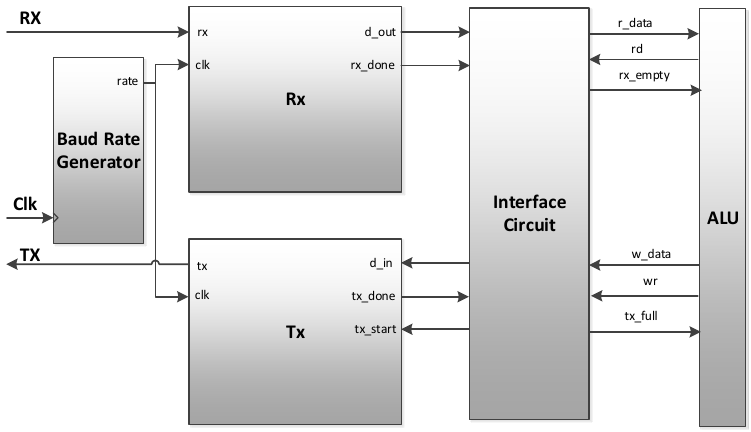
\includegraphics[scale=0.6]{figure/diagrama-UART.png}
	\caption{\textit{Diagrama de bloques implementado}}
\end{figure}

\subsection{Desarrollo del trabajo}
Se definió un módulo Top, que contiene:
\begin{itemize}
    \item Modulo UART, compuesto por:
    \begin{itemize}
        \item Baud Rate Generator
        \item Transmisor (TX)
        \item Receptor (RX)
    \end{itemize}
    \item Circuito Interfaz
    \item ALU
\end{itemize}

\subsection{UART}
\subsubsection{Baud Rate Generator}Este módulo es utilizado para coordinar el muestreo de la señal recibida. Genera un tick 16 veces por Baud Rate. A partir de la entrada de clock (conociendo su frecuencia), y la velocidad de transmisión de la UART (en ese caso, 9600 baudios), genera ticks que permiten al módulo Rx trabajar con al señal de entrada.


\subsubsection{Receptor (RX)}
\begin{figure}[H] 
	\centering
	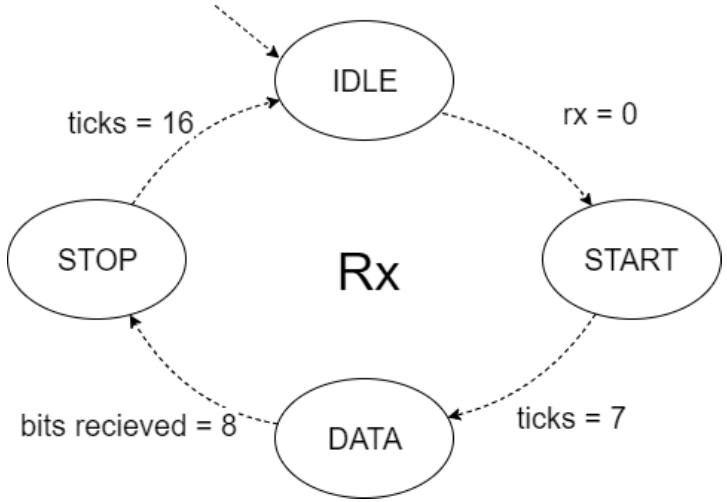
\includegraphics[scale=0.6]{figure/estados_RX.png}
	\caption{\textit{Diagrama de estados del receptor}}
\end{figure}

Es una máquina de estados que modifica su comportamiento en función de sus entradas Rx (línea de comunicación) y tick (salida del Baud Rate Generator). 

Se encuentra en estado IDLE hasta que la entrada sea un 0 lógico, lo que marca el inicio del bit de start. Luego pasa al estado START, que espera 7 ticks hasta situarse en el centro del bit de start (que dura 16 ticks), lo que sincroniza el módulo con el transmisor y asegura que el dato no se muestrea cerca del cambio de símbolo. Una vez listo, se pasa al estado DATA, en el que toma muestras del canal Rx cada 16 ticks, que marcan el centro de cada bit recibido. El paso siguiente es pasar al estado STOP, donde se lee el único bit de stop, y finalmente se pasa al estado IDLE para comenzar el ciclo nuevamente. Al finalizar la recepción de un valor, emite un pulso en una señal de fin (rx\_done\_tick).

\subsubsection{Transmisor (TX)}
\begin{figure}[H] 
	\centering
	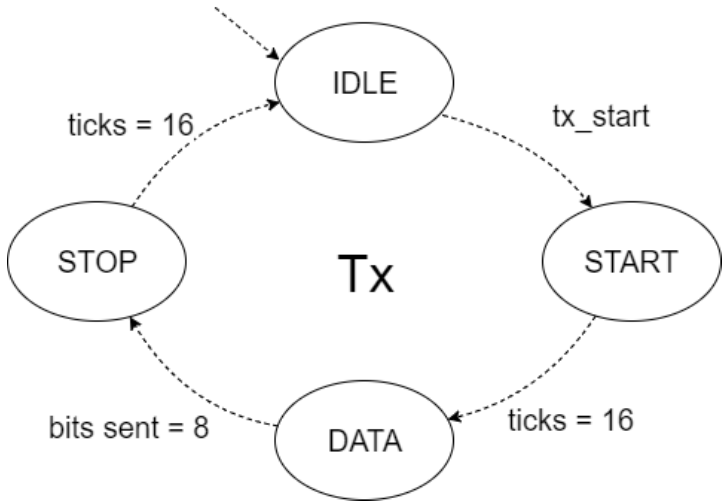
\includegraphics[scale=0.6]{figure/estados_TX.png}
	\caption{\textit{Diagrama de estados del transmisor}}
\end{figure}
Este módulo es muy similar al anterior. Posee los mismos estados, y también utiliza la señal proveniente del Baud Rate Generator para actualizar su salida (Tx) acorde a la información que se desea transmitir. Al finalizar la transmisión emite un pulso en una señal de fin (tx\_done\_tick).

Comienza en el estado IDLE, en el que envía por Tx un 1 lógico (canal inactivo). Al recibir la señal tx\_start pasa al estado START, en el que se envía un 0 lógico por el canal durante 16 ticks del Baud Rate Generator. Acto seguido se pasa al estado DATA, en el que se envía por 16 ticks cada bit del byte a transmitir, comenzando por el menos significativo. Cuando la cantidad de bits enviados sea 8 (toda la información disponible), se pasa al estado STOP, en el que se envia un bit de stop por 16 ticks del Generator. Finalmente se pasa al estado IDLE nuevamente, a la espera de más bits para transmitir.


\subsubsection{Circuito Interfaz}
\begin{figure}[H] 
	\centering
	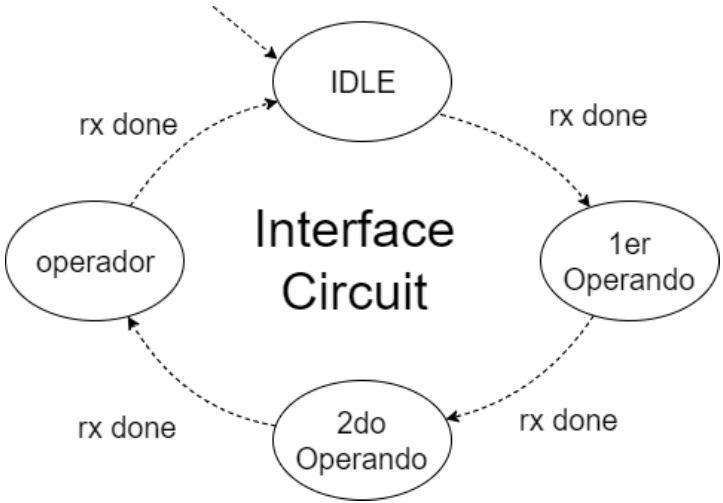
\includegraphics[scale=0.6]{figure/estados_IC.png}
	\caption{\textit{Diagrama de estados del circuito interfaz}}
\end{figure}
Permite comunicar la ALU con el módulo UART. Recibe los bytes de Rx, los almacena en tres registros (dos para los operandos, uno para el operador), y una vez tiene todos los valores, obtiene el resultado de la ALU. Seguidamente comunica al módulo Tx que el valor está listo, y lo envía mediante un bus de 8 bits.

\newpage
\subsubsection{ALU}
El módulo ALU es el desarrollado en el primer práctico. Es puramente combinacional, con dos entradas para operandos, una entrada para el operador y una salida con el resultado de la operación.

\begin{figure}[h] 
	\centering
	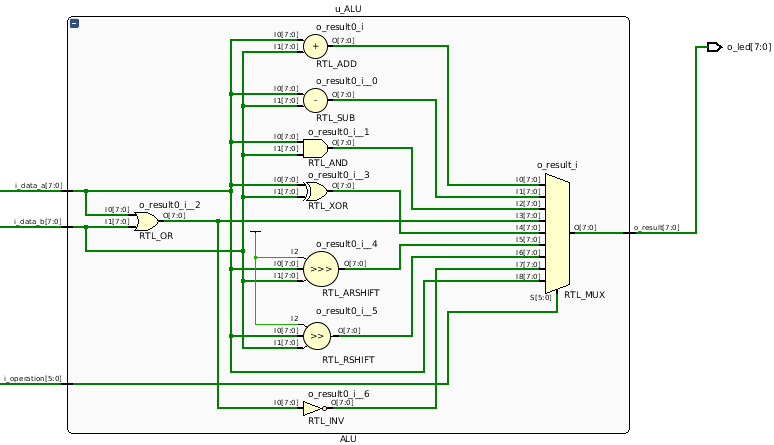
\includegraphics[scale=0.6]{figure/rtl-alu.png}
	\caption{\textit{Estructura RTL del módulo ALU obtenida de la herramienta Verilog}}
\end{figure}


\section{Simulación de los módulos}
Se realizaron las siguientes simulaciones para comprobar el correcto funcionamiento de cada uno de los bloques del sistema.

\subsection{Top\_UART}
Se comprueba el reset y que el sistema devuelva el resultado correcto cuando se ingresan operandos y códigos de operación determinados.
\begin{figure}[h]
    \centering
    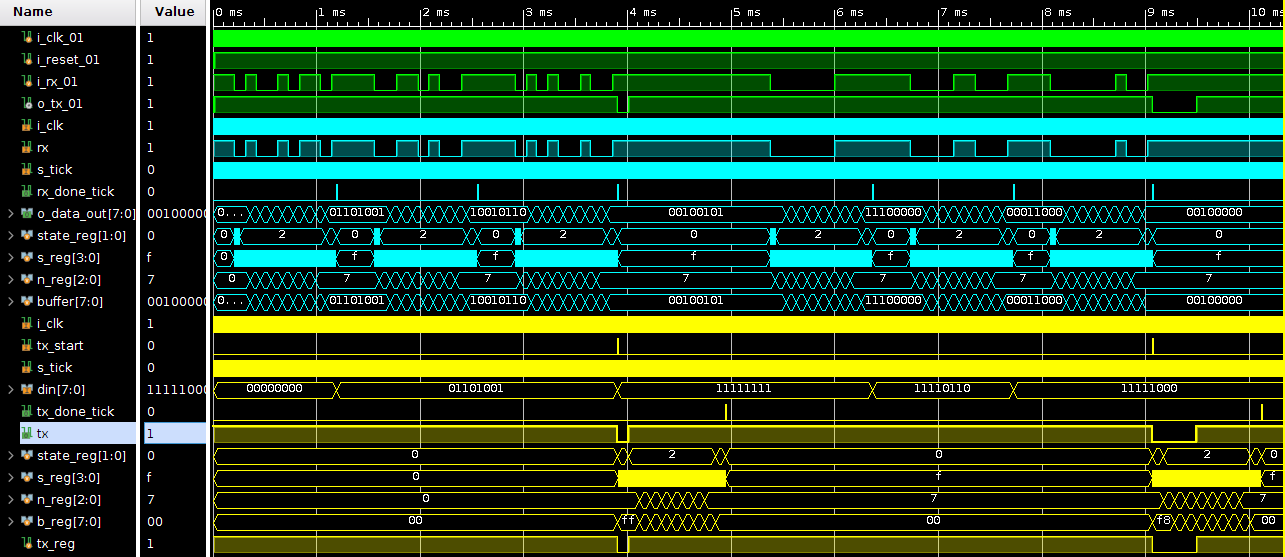
\includegraphics[width=\textwidth]{figure/top_uart.png}
    \caption{\textit{Simulación del top\_UART}}
    \label{fig:tb_top}
\end{figure}

\subsection{Baud Rate Generator}
Se comprueba la generación de los ticks con el intervalo correcto con respeto a los parámetros de entrada.

\begin{figure}[H]
    \centering
    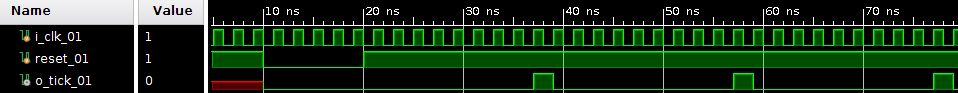
\includegraphics[width=\textwidth]{figure/tb_brg.png}
    \caption{\textit{Simulación del módulo Baud Rate Generator}}
    \label{fig:tb_brg}
\end{figure}

\subsection{Receptor (RX)}
Se envían bits y se comprueba el pasaje entre los estados del módulo y las salidas en cada uno de dichos estados. Se envían tramas correctas e incorrectas.

\subsection{Transmisor (TX)}
Se ingresa un valor a transmitir y se eleva en alto el bit de Tx\_start. Se comprueba el pasaje entre los estados del módulo y las salidas en cada uno de dichos estados.


\subsection{Circuito Interfaz}
Permite verificar el comportamiento de la interfaz y la ALU. Simula la entrada de tres valores desde Rx (operandos y operador), y permite ver que efectivamente son recibidos por la unidad aritmética.

\subsection{ALU}
Se comprobaron que el modulo sea capaz de realizar correctamente las operaciones, recibiendo los operandos y el operador para generar la salida esperada.

\section{Interface PC}
Para probar el funcionamiento de todo el proyecto, se programó un script en Python que se comunica con la FPGA mediante conexión USB, utilizando la librería PySerial. El script espera dos operandos y un operador, y una vez tenga los tres valores los transmite a la placa, mostrando el resultado en pantalla.

\begin{figure}[H]
    \centering
    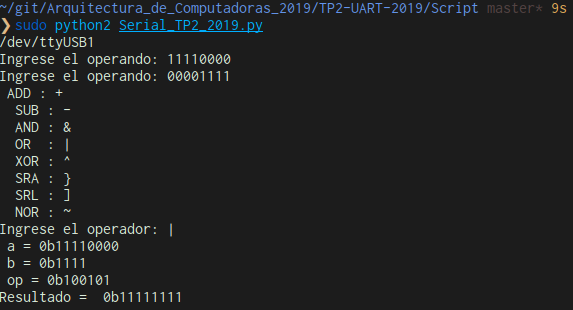
\includegraphics[width=\textwidth]{figure/scriptPython.png}
    \caption{\textit{Prueba de funcionamiento en Python}}
    \label{fig:scriptPython}
\end{figure}

\newpage
\section{Conclusión}
Una vez terminado el práctico, a través de la herramienta Vivado se
obtuvieron las especificaciones en la utilización de los recursos de la FPGA y en la potencia que consume dicho circuito instanciado. Además, en este práctico se afianzaron los conceptos en cuanto al lenguaje de descripción de hardware Verilog, incluyendo nuevos conceptos (en el contexto de verilog) como por ejemplo las maquinas de estados.

Se logro exitosamente realizar una comunicación anacrónica en serie entre la computadora y el sistema desarrollado en FPGA, pudiendo enviar operaciones simples de aritmética al modulo ALU y recibiendo el resultado de dichas operaciones en la computadora conectada.


\begin{figure}[H] 
	\centering
	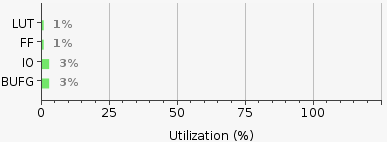
\includegraphics{figure/utilizacion-UART.png}
	\caption{\textit{Utilización de la FPGA}}
\end{figure}

\end{document}

